\documentclass{article}

\usepackage{multicol}
\usepackage{lipsum}
\usepackage{graphicx}
\graphicspath{{images/}}
\usepackage{blindtext}
\usepackage{subfiles} % Best loaded last in the preamble
\usepackage[dvipsnames]{xcolor}
\usepackage[T1]{fontenc}
\usepackage{setspace}
\usepackage{float}
\usepackage{array}

\setlength{\columnsep}{1cm}

\usepackage{fullpage, tikz}
\usepackage{eso-pic}
%\AddToShipoutPictureBG{%
%	\begin{tikzpicture}[remember picture, overlay]
%		\node[opacity=.4, inner sep=0pt]
%		at(current page.center){
\includegraphics[width=8.5in, height=11in]{images/background}};
%	\end{tikzpicture}%
%}

\usepackage[margin={1.5cm,1.5cm}]{geometry}

\newcommand\BackgroundPic{%
	\put(0,0){%
		\parbox[b][\paperheight]{\paperwidth}{%
			\vfill
			\centering
			%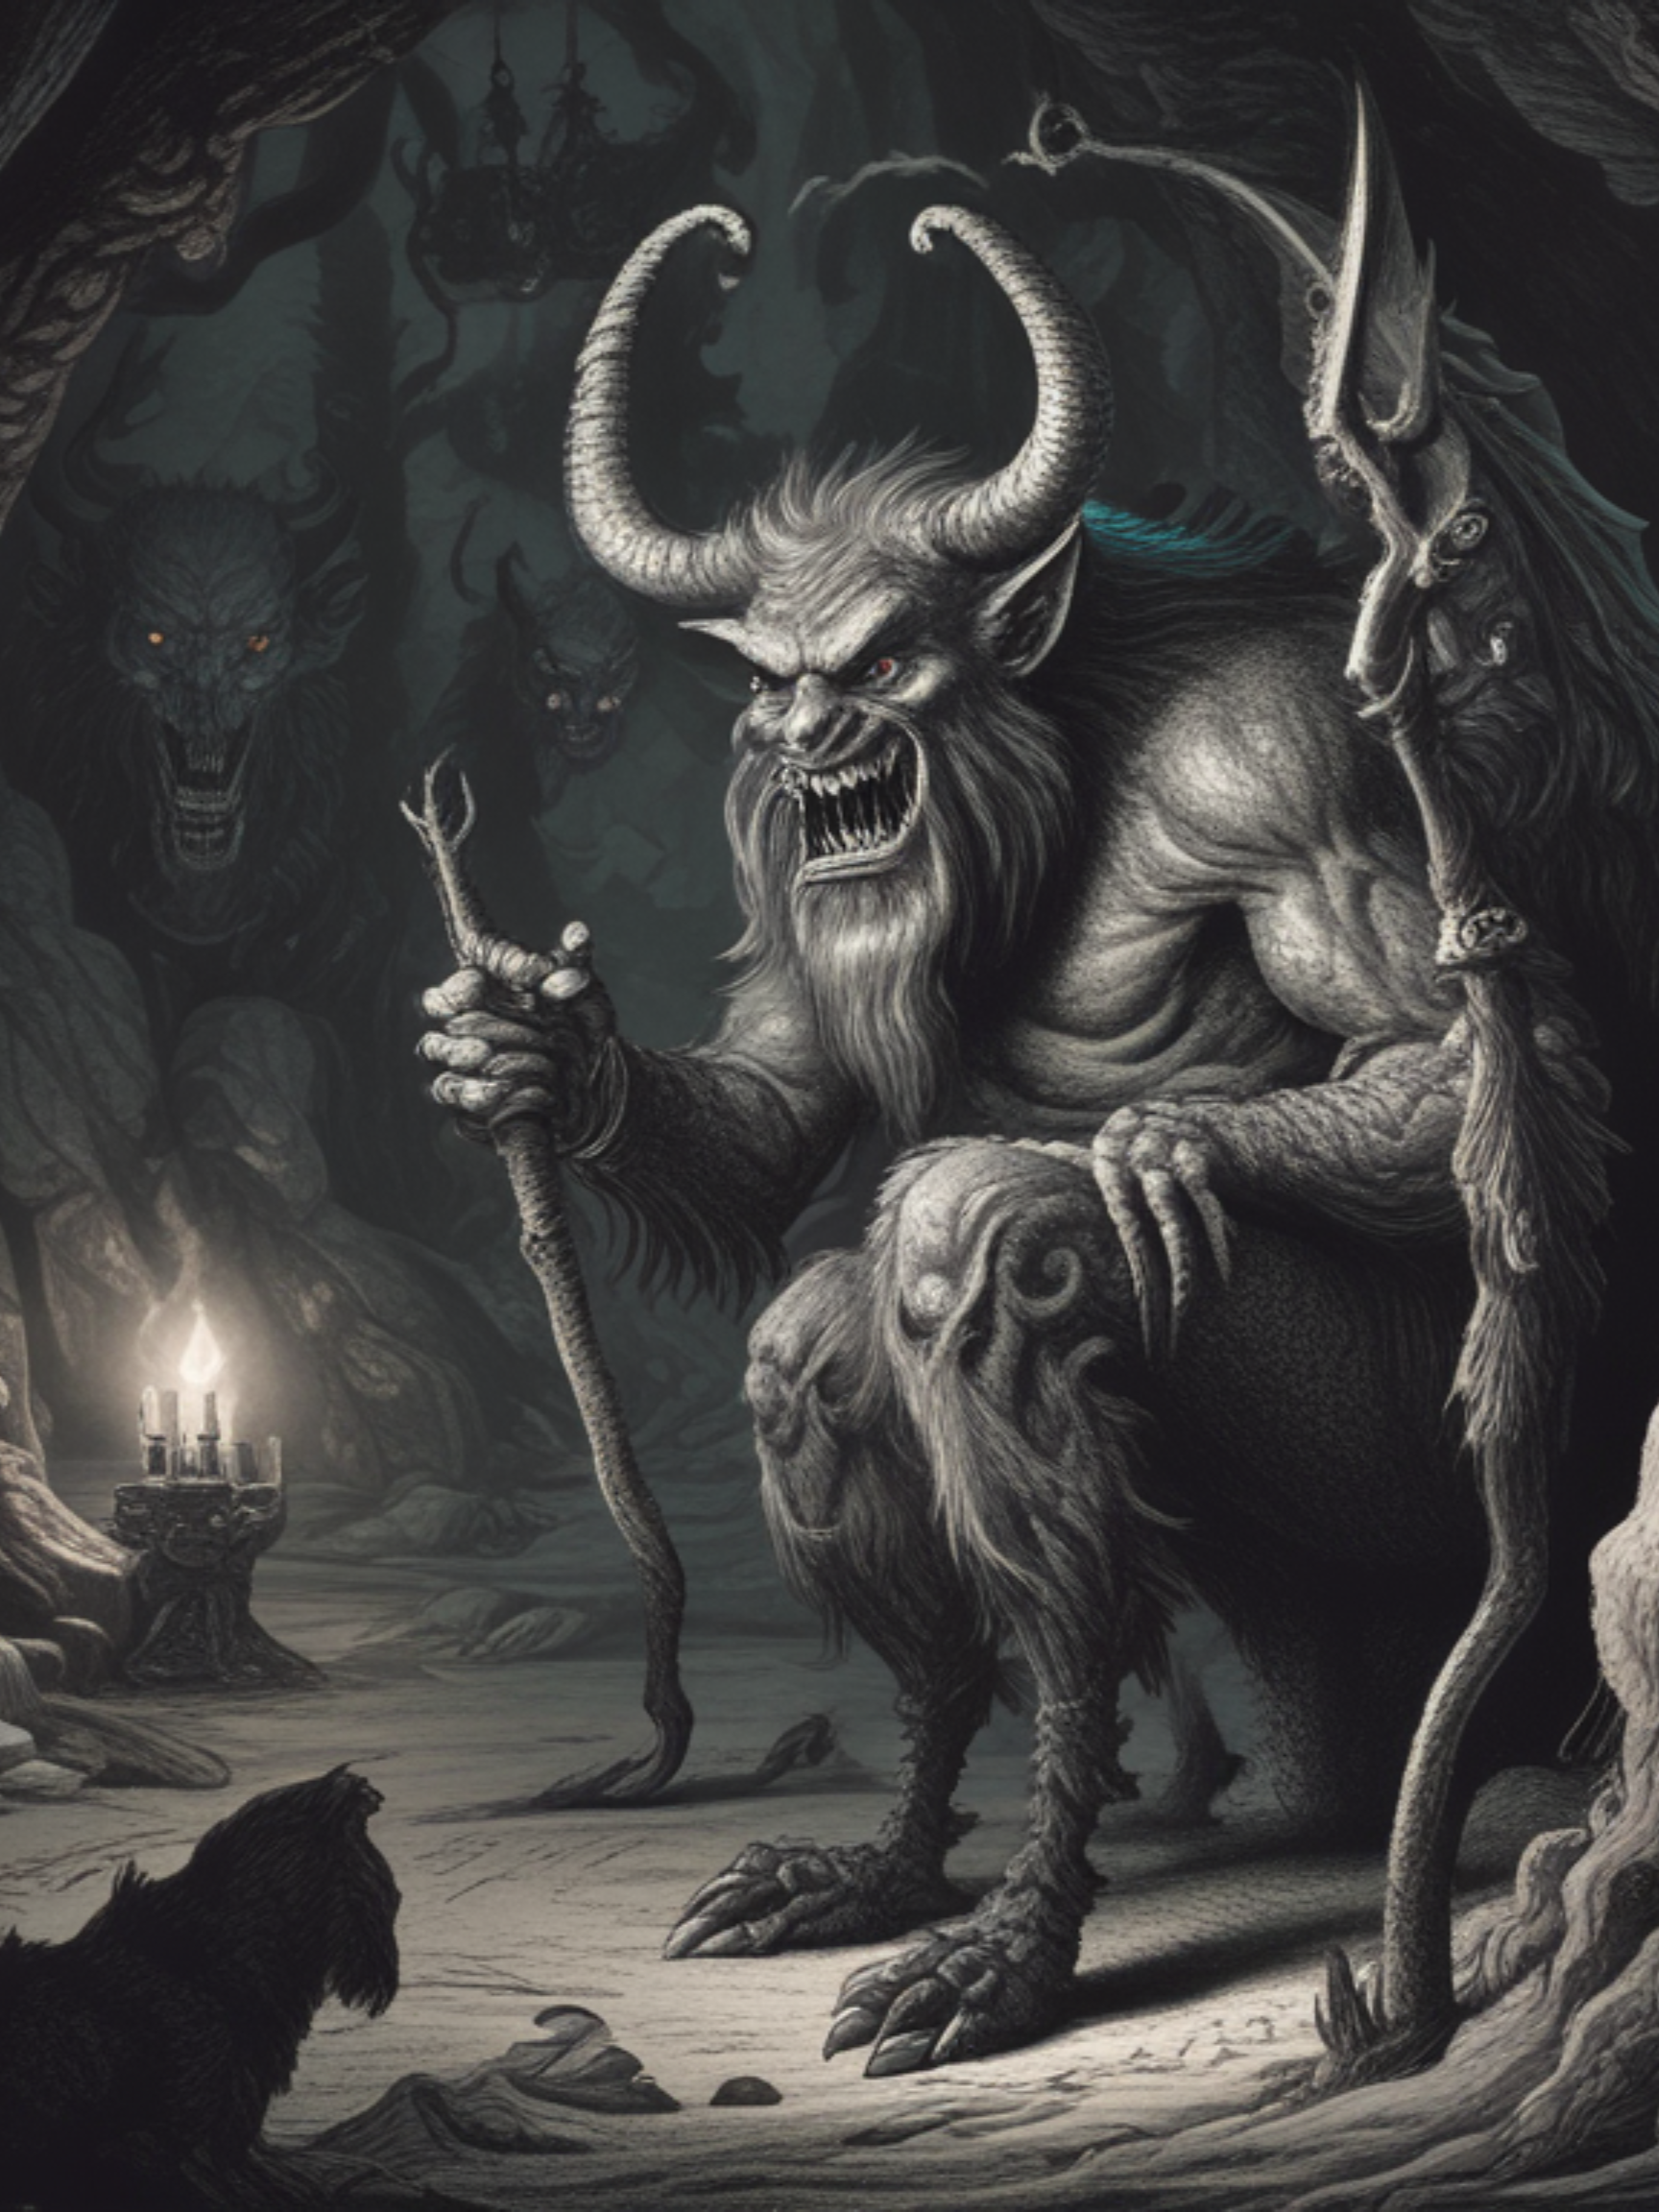
\includegraphics[width=\paperwidth,height=\paperheight]{images/cover.png}%
			\vfill
}}}

\title{\color{black}\textsc{\Huge The Frosthaven Festival }}
\date{ }


\setlength\fboxsep{8pt}

\begin{document}
	\AddToShipoutPicture*{\BackgroundPic}
	\maketitle
	\pagebreak
	\begin{multicols*}{2}
	\section{Introduction}
	
	\subsection*{Overview}
	\emph{Krampus's Vengence} one-off adventure is meant to be played with a group of 5 players at level 5. The adventure is meant to be completed in one session.
	
	It is a Christmas inspired story with familiar themes and characters. The plot of the adventure is set in the mountain town of Frosthaven during the annual winter solstice festival. Krampus, the evil goat-man, attempts to disrupt the celebrations and places the town in a snow avalanche. The players must solve puzzles and defeat Krampus to win the adventure. 
	
			\colorbox{GreenYellow}{\begin{minipage}{0.4\textwidth}
\subsubsection*{Key NPCs}
\begin{description}
	\item[The Frost King Armine] The king of the mountain village of Frosthaven.
	\item[Flambard Gamgee] Proprietor of the Frostmint Inn.
	\item[Krampus] The goat-man evil demon attempting to disrupt the winter festival. 
\end{description} 
\end{minipage}}
\break

\subsection*{Adventure Hook}

	The adventure starts as the players arrive in Frosthaven. The atmosphere is cheerful and busy, with people preparing for the three day festivities. The villagers are buzy preparing the food, music, and lights for the celebration. As the sun sets over the mountains, the town's mayor makes a speech and begins to ring the town bell. The watching crowd goes silent... A moment later, another bell is heard from within the castle courtyard, and suddenly the crowd erupts into celebration, cheering, singing, and dancing.
	
	\colorbox{lightgray}{\begin{minipage}{0.4\textwidth}
\subsubsection*{Lore}
The annual winter solstice festival in Frosthaven is a three day celebration that includes many feasts, music, and gift giving.  On the first day, the inhabitants of Frosthaven prepare a big feast for the town, and ring the bell (the Town Bell) in the town square to declare the beginning of the festival. A second bell in heard from within the castle walls indicating that the Frost King himself is planning the descend down into town to join the celebration, baring gifts for the town.

On the second day, the town bell is brought into the castle courtyard, joining the King's Bell, and are rung together in unison. The Frost king joins the townsfolk, gifts are distributed and another feast culminates the celebration. Finally, the third day is a day of rest and quiet meditation on thankfulness. 

The town bell is adorned with runes symbolizing the festival. Legends claim that placing the wrong rune-stones onto the bell can summon evil spirits, including Krampus.
\end{minipage}}
\break

	As the evening winds down, the players arrive at the Frostmint Inn, the main tavern establishment in the town. As they enjoy a late night drink, the tavern's proprietor informs them that a very important foreign dignitary arrived unexpectedly and they do not have enough rooms to accommodate all the players. Reservations were made to ensure that each player had their own room but the dignitary and his aids will take up two extra rooms. The players will have an opportunity to protest this (intimidation, or persuasion, or other means) or accept to room in groups. Make sure to keep track of who is sleeping in which room.
	
	As everyone goes to sleep, an event occurs in the middle of the night. A perception check should be performed by each player to determine which player(s) wakes up. The players are woken up to a small earthquake growing in intensity. Looking out the window reveals an avalanche headed towards the town. Awake players will have a short amount of time to warn the rest of the party. When the avalanche hits the town, pick two rooms which get hit, and ironically, the two rooms meant for the dignitaries if the players are there. Players in rooms hit by the avalanche will need to make a \textbf{DC 15 acrobatic} check (with disadvantage if they are still asleep) to determine if they escape the destruction or take \textbf{2d6} damage.
	
	\colorbox{lightgray}{\begin{minipage}{0.4\textwidth}
\subsubsection*{Snow Fall}
Periodically, snow falls from the dome ceiling, requiring the players to do a \textbf{DC 15 acrobatic} check or take \textbf{2d6 cold and bludgeoning damage}. Targeted players can be determined randomly and the frequency of this event can be at the discretion of the DM. The area of effect is 15ft in diameter.
\end{minipage}}
\break
	
	At this point, the town of Frosthaven is completely under the snow, except for the town square with appears to be protected by a magical bubble, and looks like a big dome of snow. Many of the buildings are completely or partially enveloped and iced in. The will need to find a way to escape before the entire dome collapses on the town. 

\section{The Frosthaven Town Square}
	The bell in the town square is the centerpiece of the puzzle. The bell is a large mounted structure on four pedestals which contain slots where rune stone tablets are placed. The tablets that were previously placed in the slots have been scattered around the town square during the earthquake and avalanche. The players must find the run stone tablets around the town square and place the correct ones onto the bell's pedestal slots to open a passage way to the castle courtyard.
	
	\begin{figure*}
	\centering
	\includegraphics[width=0.9\textwidth]{images/frosthaven_town}
	\caption{Frosthaven Town Square}
	\end{figure*}
	
	
	
	There will be eight tablets to be found around the town center, but only four of those can be placed into the bell's slots. Normally, the traditional runes would occupy those slots, but to open the passage to the castle courtyard and confront Krampus, the players will have to have to use the Krampus runes. The location and order the players find the tablets can be left to the discretion of the DM, however the recommended locations should be the following: One by the well, two in the library, two in the blacksmith's shop, two in the cemetery, and the last one is in the butcher's shop. The players will need to thoroughly investigate each location to recover all the clues.
	
	\begin{figure*}
	\centering
	
\includegraphics[width=0.2\textwidth]{images/bell}
	
\includegraphics[width=0.2\textwidth]{images/giftbox}
	
\includegraphics[width=0.2\textwidth]{images/christmas-tree}
	
\includegraphics[width=0.2\textwidth]{images/santa-hat}
	\caption{Traditional Runes}
	\end{figure*}
	
	\begin{figure*}
	\centering
	
\includegraphics[width=0.2\textwidth]{images/goat}
	
\includegraphics[width=0.2\textwidth]{images/whip}
	
\includegraphics[width=0.2\textwidth]{images/snake}
	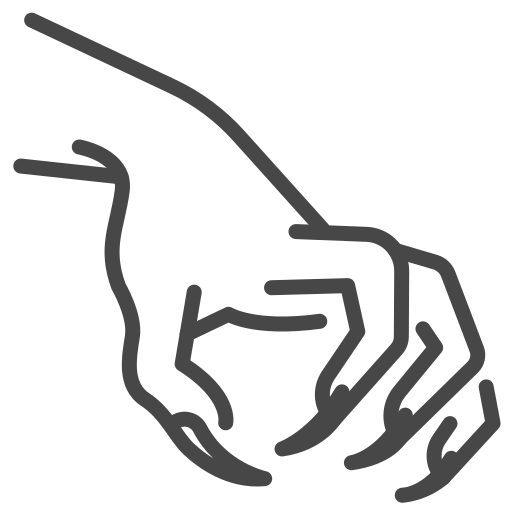
\includegraphics[width=0.2\textwidth]{images/hand}
	\caption{Krampus Runes}
	\end{figure*}	
	
\begin{description}
\item[The Frostmint Inn] No runes found here, but the frozen body of the proprietor.
\item[Town Square] Center of the town, location of the bell, and a rune by the well.
\item[Blacksmith's] Contains two runes and possibly three or four magical items and the frozen body of the blacksmith and his apprentice. They apparently had been working late putting the finishing touch on the gifts for the Frost King. 
\item[Library] Contains two runes, the Wand of Eternal Flame, and one or two extra magical items and the frozen body of the librarian. He can be found at slumped over his desk frozen. It appears as though he had been up late studying. His notes read ``... during the reign of the Frost King Thodor, the star of Ark'rumus appears brighter and slightly above the Great Bell constellation. The ringing of the bell ultimately ushered the terrifying return of the desolate and evil...'' The rest of the text is damaged and illegible.
\item[Butcher's Shop] Contains a rune, and the frozen bodies of the butcher, and two other villagers. They appear to have been enjoying a late night drink before the avalanche. An investigation check reveals that the integrity of the structure has been compromised and is about to collapse. If the player(s) spend too much time in the butcher's shop, it eventually collapses. A dexterity check will be require to see if they escape or take 2d8 damage, and be trapped. Other players will need to help them to get out.
\item[Cemetery] Contains a rune. If the players fail the rune puzzle, two zombies will rise from the cemetery.

\end{description}

	Each location should have features of interest and potentially some magical items usable by the players. Preferably, players should be able to each find a magical item usable by their characters. Refer to the table below for ideas of items players can find.
	
	\begin{table}[H]
		\begin{tabular}{|m{7.5em}|m{15em}|}
			\hline
			\textbf{Item} & \textbf{Description} \\
			\hline
			\hline
			Wand of Eternal Flame & This wand has 8 firebolt charges. Its wielder can choose to expend 1 to 3 charges at a time, doing 1d10 per charge. Gain the \emph{Eternal Flame} cantrip, which produces a flame capable of melting snow, the target within melee range must succeed on a Dexterity saving throw or take 1d8 fire damage \\ 
			\hline
			Armor of Resistance (Cold) & Gain cold resistance (half damage)  \\
			\hline
			Weapon +1 & Any weapon with +1 \\
			\hline
			Weapon +2 & Any weapon with +2 \\
			\hline
			Flame Tongue Weapon & Deals an extra 2d6 Fire damage on a hit.  \\ 
			\hline
			Snow Ring & Wielder can turn into snow and move around undetected (disadvantage on perception) in areas covered with snow. \\
			\hline
			Potion of Healing & Regains 2d4 + 2 hit points. \\
			\hline
			Potion of Greater Healing & Regains 2d8 + 2 hit points. \\
			\hline
		\end{tabular}
	\end{table}


\subsection*{Encounter}
Once the party has found all the rune tablets, they will need to place the Krampus runes into the slots. If they choose the wrong combination of runes, the townsfolk are not saved, and turn into frost zombies. To begin the encounter, the players must place the runes in the slots and ring the bell. The Krampus runes will light up and the traditional runes will burn up and the encounter begins. If the players chose incorrectly they will need fight both the snow owlbear and zombies. The number of zombies can be adjusted as needed but it should be broken down as follows: blacksmith (2), library (1), butcher's shop (3), cemetery (2).

\subfile{../../monsters/snow-owlbear}
\subfile{../../monsters/frost-zombie}

Once the Snow Owlbear is defeated, the encounter is completed and the way to the castle courtyard opens up once the correct runes have been placed into the bell's slots.

\section{Castle Courtyard}

	\begin{figure*}
	\centering
	\includegraphics[width=0.9\textwidth]{images/castle_courtyard}
	\caption{Frosthaven Town Square}
	\end{figure*}
	
As the players enter the courtyard they can see and hear the Frost bell ringing in the center of the castle courtyard. There is a general feeling of uneasiness and evil concentrated in this area. Rats can be seen wandering around the courtyard (later will turn into imps). The players should notice a rail which connects to the town square, which allows the bell to be moved into the castle courtyard. 

To begin the battle against Krampus, the players will need to drag the town bell into the castle courtyard and ring the bell. Once the bell begins ringing, eventually the two bells begin ringing in sync. All of sudden, the snow bubble around the town collapses onto the castle 
courtyard. Everything goes dark, except for a few torches. An evil laugh can be heard echoing in the dark all around in the courtyard.

\colorbox{lightgray}{\begin{minipage}{0.4\textwidth}
\subsubsection*{Krampus Origins}
Krampus is usually featured as a man with horns with one grotesque human foot and one foot of a goat. He is typically covered in black hair and has a very long snake or dragon-like tongue. Krampus carries chains, thought to symbolize the binding of the Devil by the Church. He thrashes the chains for dramatic effect. The chains are sometimes accompanied with bells of various sizes.

Krampus will carry a bundle of birch branches with which he occasionally swats children. The birch branches are replaced with a whip in some representations. On Christmas Eve, Krampus travels with a sack or a basket strapped to his back; this is to cart off evil children for drowning, eating, or transport to Hell. Some of the older versions make mention of naughty children being put in the bag and taken away.
\end{minipage}}
\break

Krampus is a horned hairy goat-man devil, and is basically a \emph{Barbed Devil} but instead of fire, his damage and resistance types are cold, and is weak against fire. The same applies to his imps. The players will need to defeat Krampus to free the town of Frosthaven.

\subfile{../../monsters/barbed-devil}
\subfile{../../monsters/imp}
		
\section{Conclusion}

Once Krampus is defeated, snow bubble collapses over the town, knocking the players unconscious. They wake up back in their respective rooms in the Frostmint Inn, as if nothing had happened. The celebrations for the solstice festival continue and the townsfolk appear clueless to the events that just occurred. The town bell is pulled into the courtyard, the bells ring as the people cheer and the Frost King makes an appearance. One of the king's guards approaches the players and informs them that the King has requested an audience with them.

The king, apparently aware of the events that unfolded, thanks the players and gives each of them necklaces and honors the players as the saviors of Frosthaven.

You can include a more detailed or different ending here as needed.

	\pagebreak
\end{multicols*}
	
\end{document}
